\documentclass[reprint,amsmath,amssymb,aps,prapplied,superscriptaddress,floatfix]{revtex4-2}
\usepackage{graphicx}

\usepackage{bm}

\usepackage{tikz}
\usetikzlibrary{arrows.meta,decorations.pathmorphing,calc}
\usepackage[colorlinks=true,linkcolor=blue,citecolor=blue,urlcolor=blue]{hyperref}
\newcommand{\todo}[1]{\textcolor{red}{[TODO: #1]}}
\newcommand{\dBus}{dB/$\mu$s}

\begin{document}

\title{Comb-pumped backward Brillouin storage of frequency-bin photons in thin-film lithium niobate:\\ delay figures of merit and a phase-matching limit on mode selectivity}

\author{\todo{author list}}
\affiliation{\todo{affiliations}}

\date{\today}

\begin{abstract}
We analyze, using simulations and closed-form estimates only, a backward stimulated-Brillouin-scattering (SBS) memory in thin-film lithium niobate (TFLN) pumped by an electro-optic frequency comb, proposed as an all-optical, transducer-free buffer for frequency-bin photons. With measured TFLN parameters the acoustic delay loss at 4~K is 2.2~\dBus{}, which is $78\times$ and $12\times$ below record and material-limited TFLN optical delay lines (169 and 26~\dBus{}), and 1~$\mu$s of acoustic delay occupies 3.1~mm. Off-chip fiber is still $53\times$ better in loss (0.04~\dBus{}) but requires 204~m. A full photon--phonon swap needs 16~mW of peak pump for 10-MHz photons and 1.55~W for 100-MHz photons, which restricts the scheme to narrowband photons. A thermal-noise model excludes single-photon operation at room temperature and gives a noise-limited qubit fidelity above 0.9 for storage up to 40~ns at 4~K. At 20~mK the fidelity stays above 0.99 up to 10~$\mu$s, under the untested assumption that the 4-K acoustic loss carries over to millikelvin temperatures. A single-acoustic-mode model predicts that the comb-line amplitudes and phases select which frequency-bin superposition is stored, with selectivity 0.9988 for eight bins. We show, however, that this local model fails for backward SBS. Bins spaced by $\Delta$ write phonon gratings whose wave vectors differ by $2\Delta n_g/c$ (964~rad/m for 10-GHz bins), and these gratings are mutually orthogonal over the meter-scale collision region that nanosecond photons require. A space--time simulation confirms that the two-bin selectivity collapses to 0.50. What survives is a bin-diagonal memory with per-bin programmable swap, phase, and read time. It supports re-timing and synchronization of photons across bins, but it cannot remap frequency or select superpositions.
\end{abstract}

\maketitle

%=====================================================================
\section{Introduction}
%=====================================================================
Frequency-bin encoding places many qubit or qudit modes in a single waveguide mode and is naturally phase stable~\cite{Lu2023Review}. Programmable frequency-bin gates have been demonstrated with electro-optic (EO) quantum frequency processors~\cite{LukensLougovski2017,Lu2018PRL}, EO frequency beam splitters on TFLN~\cite{Hu2021Nature,Yang2026QFP}, and temporal-mode-selective sum-frequency generation in TFLN quantum pulse gates~\cite{Babel2026QPG}. None of these devices can store a photon. On-chip TFLN storage has so far relied on optical recirculation~\cite{Ekici2023} or long delay lines~\cite{Song2023ODL}, whose loss per unit delay is set by the optical propagation loss~\cite{ZhuX2024PRJ,ShamsAnsari2022}.

Brillouin light storage avoids this limit by transferring the optical signal to a traveling acoustic wave that moves $\sim 10^5$ times more slowly than light. It was demonstrated in fiber~\cite{ZhuGauthierBoyd2007} and on a chalcogenide chip~\cite{Merklein2017}, extended to multiple wavelength channels without crosstalk~\cite{Stiller2019}, to phonon refreshing~\cite{Stiller2020}, to storage over 100 pulse widths~\cite{Stiller2024}, to cryogenic fiber~\cite{Geilen2024}, to phase-encoded data~\cite{Saffer2025}, and to polarization multiplexing~\cite{Zeng2026}. Quantum-regime analyses now predict optoacoustic entanglement~\cite{ZhuGenesStiller2024} and a solid-state Brillouin quantum memory~\cite{ZhuGenesStiller2026}. In parallel, SBS has been observed in TFLN waveguides~\cite{Ye2023SAW,Ye2025SciAdv,Rodrigues2025,Haerteis2025}, and gigahertz phononic waveguides with sub-dB/mm loss at 4~K have been reported in lithium niobate on sapphire~\cite{Mayor2021}.

This paper evaluates whether these ingredients can be combined into a \emph{phononic frequency-bin buffer} (PFB) in TFLN. In this all-optical scheme an EO comb supplies the write and read pumps, and no interdigital transducer (IDT) is needed. The original premise of the concept was that the comb-line amplitudes and phases choose \emph{which} frequency superposition is written into the phonon, and that a later read pulse with an arbitrary comb combination releases it on demand. This would provide time--frequency permutation and photon synchronization. We quantify the delay figures of merit, pump power, and thermal-noise-limited fidelity. We then show that the premise of superposition selection does not survive the phase-matching geometry of backward SBS, and we identify the reduced functionality that remains.

All numbers in this work are simulations or analytic estimates built on literature parameters; no device was fabricated or measured. Parameters and their status are collected in Table~\ref{tab:params}.

%---------------------------------------------------------------------
\begin{figure}[t]
\centering
\resizebox{\columnwidth}{!}{%
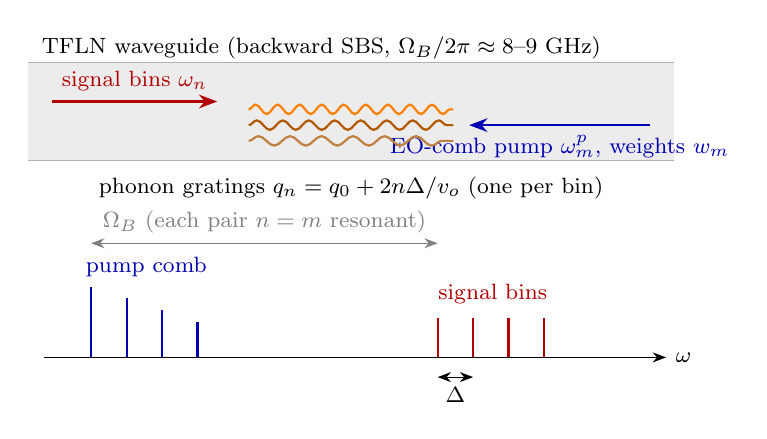
\begin{tikzpicture}[x=1cm,y=1cm,>=Stealth,font=\footnotesize]
 % waveguide
 \fill[gray!15] (0,0) rectangle (8.2,1.25);
 \draw[gray!60] (0,0) -- (8.2,0); \draw[gray!60] (0,1.25) -- (8.2,1.25);
 \node[anchor=west] at (0.05,1.43) {TFLN waveguide (backward SBS, $\Omega_B/2\pi\approx 8$--9~GHz)};
 % signal
 \draw[->,thick,red!70!black] (0.3,0.75) -- (2.4,0.75) node[above,pos=0.5]{signal bins $\omega_n$};
 % pump
 \draw[<-,thick,blue!70!black] (5.6,0.45) -- (7.9,0.45) node[below,pos=0.5]{EO-comb pump $\omega^{p}_m$, weights $w_m$};
 % gratings
 \foreach \y/\p/\c in {0.65/0.28/orange, 0.45/0.33/orange!70!black, 0.25/0.40/brown} {
   \draw[\c,thick,decorate,decoration={snake,amplitude=0.6mm,segment length=\p cm}] (2.8,\y) -- (5.4,\y);}
 \node[align=center] at (4.1,-0.35) {phonon gratings $q_n=q_0+2n\Delta/v_o$ (one per bin)};
 % spectrum inset
 \begin{scope}[shift={(0.2,-2.5)}]
 \draw[->] (0,0) -- (7.9,0) node[right]{$\omega$};
 \foreach \i in {0,1,2,3} {\draw[blue!70!black,thick] (0.6+0.45*\i,0) -- (0.6+0.45*\i,{0.9-0.15*\i});}
 \node[blue!70!black] at (1.3,1.15) {pump comb};
 \foreach \i in {0,1,2,3} {\draw[red!70!black,thick] (5.0+0.45*\i,0) -- (5.0+0.45*\i,0.5);}
 \node[red!70!black] at (5.7,0.8) {signal bins};
 \draw[<->] (5.0,-0.25) -- (5.45,-0.25) node[midway,below]{$\Delta$};
 \draw[<->,gray] (0.6,1.45) -- (5.0,1.45) node[midway,above]{$\Omega_B$ (each pair $n=m$ resonant)};
 \end{scope}
\end{tikzpicture}}
\caption{Concept of the comb-pumped backward-SBS frequency-bin buffer. Signal bins $\omega_n=\omega_0+n\Delta$ meet a counter-propagating EO-comb pump with lines $\omega^p_m=\omega_m-\Omega_B$ and complex weights $w_m$. Only pairs $n=m$ drive the phonon resonantly. Because backward SBS requires $q\simeq k_s+|k_p|$, pair $n$ writes a grating with wave vector $q_0+2n\Delta/v_o$ (Sec.~\ref{sec:phase}).}
\label{fig:concept}
\end{figure}

%=====================================================================
\section{Concept and model}\label{sec:model}
%=====================================================================
\subsection{Geometry and coupled-mode equations}
Signal bins $\omega_n=\omega_0+n\Delta$ ($n=-\tfrac{N-1}{2},\dots,\tfrac{N-1}{2}$; $\Delta/2\pi=10$~GHz assumed) propagate in $+z$ with group velocity $v_o=c/n_g$. A pump comb with lines $\omega^p_m=\omega_m-\Omega_B$, normalized complex weights $w_m$ ($\sum_m|w_m|^2=1$), and common envelope $p(z+v_ot)$ propagates in $-z$. Pair $(n,m)$ beats at frequency $\Omega_B+(n-m)\Delta$ and wave vector $q_{nm}=k_n+|k^p_m|\simeq q_0+(n+m)\Delta/v_o$. On nanosecond time scales the phonon envelope $B(z,t)$ is effectively local, because it moves only $v_{ac}t\sim 3~\mu$m in 1~ns. In a frame rotating at $(\Omega_B,q_0)$ and $(\omega_n,k_n)$, the envelopes obey
\begin{align}
(\partial_t+v_o\partial_z)A_n &= -i\,g\,p\sum_m w_m e^{-i\Phi_{nm}}B,\label{eq:A}\\
\partial_t B &= -i\,g\,p\sum_{n,m} w_m^{*}e^{i\Phi_{nm}}A_n-\tfrac{\Gamma}{2}B,\label{eq:B}\\
\Phi_{nm}&=\kappa\,(n+m)\frac{\Delta}{v_o}z-(n-m)\Delta t,\label{eq:phi}
\end{align}
where $\Gamma$ is the phonon energy decay rate. The physical backward-SBS case is $\kappa=1$. Setting $\kappa=0$ removes the spatial phase and gives the \emph{local}, single-acoustic-mode model used in the original concept study [Sec.~\ref{sec:local}]. The source scripts also include the small Brillouin-frequency dispersion $\epsilon=2n_gv_{ac}/c=4.76\times10^{-5}$, which detunes pair $n$ by $n\epsilon\Delta$ (2$\pi\times0.48$~MHz per 10-GHz bin).

\subsection{Pump power for a full swap}
Using the standard result that $G_B\Gamma$ is independent of temperature, we take the coupling rate as $g^2=G_B\Gamma v_oP/4$. The counter-propagating overlap time is $\tau_w/2$. A full photon$\to$phonon swap ($g\tau_w/2=\pi/2$) then requires a peak pump power
\begin{equation}
P_\pi=\frac{4\pi^2}{G_B\Gamma v_o\tau_w^2},\label{eq:Ppi}
\end{equation}
which we evaluate with $\tau_w=1/B$ for photon bandwidth $B$. Equation~\eqref{eq:Ppi} assumes that the signal and pump collide completely inside the waveguide. As discussed in Sec.~\ref{sec:length}, this requires an optical interaction length of order $v_o\tau$.

\subsection{Noise-limited fidelity}
We assume ideal $\pi$-swaps. The write pulse then maps the (vacuum-plus-signal) optical mode onto the phonon and resets the phonon's thermal occupation, which then rethermalizes. The read pulse retrieves the stored excitation with efficiency $\eta=e^{-\Gamma(t+\tau_w)}$, together with $n_{\rm add}=n_{th}(1-e^{-\Gamma(t+\tau_w)})$ thermal phonons, where $n_{th}$ is the Bose occupation at 8~GHz. Each added noise quantum gives a random qubit outcome. Conditioned on a detection, the qubit fidelity is
\begin{equation}
F=\frac{\eta+n_{\rm add}/2}{\eta+n_{\rm add}}.\label{eq:F}
\end{equation}
Multi-photon events, pump heating, and spontaneous Stokes/anti-Stokes scattering of the pump are not included (Sec.~\ref{sec:limits}). We use $\Omega_B/2\pi=8.0$~GHz in $n_{th}$. The TFLN device that supplies $G_B$ operates at 8.70~GHz~\cite{Ye2023SAW}, where $n_{th}(4~{\rm K})=9.1$ instead of 9.9, so our 4-K noise estimate is slightly pessimistic.

%---------------------------------------------------------------------
\begin{table}[t]
\footnotesize
\caption{Model inputs. ``Meas.'' denotes a measured literature value. ``Assum.'' denotes an assumption of this work.}
\label{tab:params}
\begin{ruledtabular}
\begin{tabular}{p{2.9cm}p{2.2cm}p{3.0cm}}
Quantity & Value & Source / status\\ \hline
\raggedright Brillouin gain $G_B$&\raggedright 26.1~W$^{-1}$m$^{-1}$&\raggedright Meas.\ (x-cut TFLN, 8.70~GHz)~\cite{Ye2023SAW}\tabularnewline
\raggedright Brillouin linewidth (RT)&\raggedright 11.9~MHz&\raggedright Meas.~\cite{Ye2023SAW}\tabularnewline
\raggedright Brillouin shift used&\raggedright 8.0~GHz&\raggedright Assum.\ (device: 8.70~GHz)\tabularnewline
\raggedright Optical group index $n_g$&\raggedright 2.3&\raggedright Assum.\ (not sourced)\tabularnewline
\raggedright TFLN optical loss, record&\raggedright 1.3~dB/m&\raggedright From $Q_i=2.9\times10^7$~\cite{ZhuX2024PRJ}\tabularnewline
\raggedright TFLN optical loss, material&\raggedright 0.2~dB/m&\raggedright Meas.~\cite{ShamsAnsari2022}\tabularnewline
\raggedright TFLN long delay line&\raggedright 0.025~dB/cm, 30~cm&\raggedright Meas.\ (abstract)~\cite{Song2023ODL}\tabularnewline
\raggedright Fiber loss / group index&\raggedright 0.2~dB/km / 1.468&\raggedright Assum.\ (standard SMF)\tabularnewline
\raggedright Acoustic loss RT / 4~K&\raggedright 4.0 / 0.7~dB/mm&\raggedright Meas.\ at $\approx$3.4~GHz~\cite{Mayor2021}\tabularnewline
\raggedright Acoustic group velocity&\raggedright 3.1~km/s&\raggedright Meas.~\cite{Mayor2021}\tabularnewline
\raggedright Acoustic loss at 20~mK&\raggedright = 4-K value&\raggedright Assum.\ (unmeasured)\tabularnewline
\raggedright Bin spacing $\Delta/2\pi$&\raggedright 10~GHz&\raggedright Assum.\tabularnewline
\end{tabular}
\end{ruledtabular}
\end{table}

%=====================================================================
\section{Delay figures of merit}\label{sec:fom}
%=====================================================================
Figure~\ref{fig:fom} and Table~\ref{tab:fom} compare loss and physical length per microsecond of delay. Optical delay costs $\alpha v_o$, acoustic delay costs $\alpha_{ac}v_{ac}$, and a phonon limited by its Brillouin linewidth costs $(10/\ln 10)\Gamma$. With the 4-K acoustic loss of Ref.~\cite{Mayor2021}, the phononic delay costs 2.17~\dBus{}. This is a factor 78 below a TFLN optical line at the record 1.3~dB/m (169~\dBus{}) and a factor 12 below the 0.2-dB/m material limit (26~\dBus{}). The demonstrated 30-cm TFLN delay line (0.025~dB/cm)~\cite{Song2023ODL} corresponds to 326~\dBus{}. The acoustic wave travels 3.1~mm in 1~$\mu$s, whereas light in TFLN needs 130~m.

Single-mode fiber is better still. At 0.2~dB/km it costs 0.041~\dBus{}, a factor 53 below the 4-K phonon, but it requires 204~m of fiber per microsecond and chip-to-fiber coupling. The phononic route therefore offers compactness and electrically free, on-chip programmability, not lower loss than fiber. At room temperature the measured SBS linewidth of TFLN (11.9~MHz, $\sim$13~ns phonon lifetime) corresponds to 325~\dBus{}, which is worse than a TFLN optical line. The 4-K figure relies on a different, lower-frequency acoustic mode (see Sec.~\ref{sec:limits}).

\begin{figure}[t]
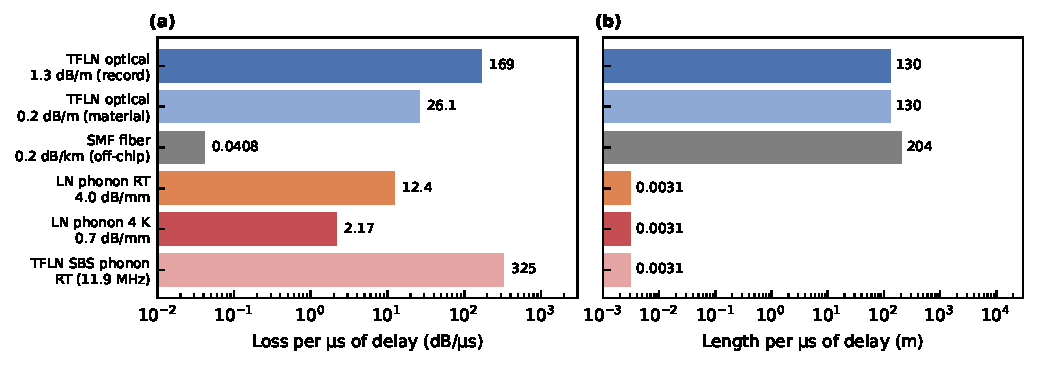
\includegraphics[width=\columnwidth]{figures/fig2_delay_fom.pdf}
\caption{(a) Loss and (b) physical length per microsecond of delay. Optical rows use $n_g=2.3$ (TFLN) or 1.468 (fiber). Acoustic rows use the 3.4-GHz loss data of Ref.~\cite{Mayor2021} with $v_{ac}=3.1$~km/s. The last row converts the measured RT Brillouin linewidth of TFLN~\cite{Ye2023SAW}. Data: \texttt{fig1\_delay\_line\_comparison.csv}.}
\label{fig:fom}
\end{figure}

\begin{table}[t]
\footnotesize
\caption{Key figures of merit (simulation/analytic).}
\label{tab:fom}
\begin{ruledtabular}
\begin{tabular}{p{4.6cm}p{3.4cm}}
Quantity & Value\\ \hline
\raggedright Phonon delay loss, 4~K (0.7~dB/mm)&\raggedright 2.17~\dBus{}\tabularnewline
\raggedright Phonon delay loss, RT (4.0~dB/mm)&\raggedright 12.4~\dBus{}\tabularnewline
\raggedright TFLN SBS phonon, RT (11.9~MHz)&\raggedright 325~\dBus{}\tabularnewline
\raggedright TFLN optical, 1.3 / 0.2~dB/m&\raggedright 169 / 26.1~\dBus{}\tabularnewline
\raggedright SMF, 0.2~dB/km&\raggedright 0.041~\dBus{}\tabularnewline
\raggedright Length per $\mu$s: acoustic / TFLN / SMF&\raggedright 3.1~mm / 130~m / 204~m\tabularnewline
\raggedright $P_\pi$ at 10 / 100 / 1000~MHz&\raggedright 15.5~mW / 1.55~W / 155~W\tabularnewline
\raggedright Interaction length $v_o\tau$ at 10 / 100~MHz&\raggedright 13~m / 1.3~m\tabularnewline
\raggedright 4~K: $\Gamma/2\pi$, $n_{th}$&\raggedright 79.5~kHz, 9.9\tabularnewline
\raggedright 4~K: $\eta(1~\mu{\rm s})$, half-efficiency time&\raggedright 0.60, 1.38~$\mu$s\tabularnewline
\raggedright 4~K: delay--bandwidth product ($\tau_w=10$~ns)&\raggedright 138\tabularnewline
\raggedright 4~K: $F>0.9$ / $F>2/3$ up to&\raggedright 40~ns / 0.36~$\mu$s\tabularnewline
\raggedright 20~mK (assumed loss): $F>0.99$ up to&\raggedright $\ge$10~$\mu$s\tabularnewline
\raggedright Local-model selectivity, $N=8$, $\tau_w=1$~ns&\raggedright 0.9988\tabularnewline
\raggedright Space--time selectivity, $N=2$, backward SBS&\raggedright 0.500\tabularnewline
\end{tabular}
\end{ruledtabular}
\end{table}

%=====================================================================
\section{Pump power, bandwidth, and interaction length}\label{sec:length}
%=====================================================================
Equation~\eqref{eq:Ppi} gives $P_\pi=15.5$~mW for $B=10$~MHz, 1.55~W for 100~MHz, and 155~W for 1~GHz [Fig.~\ref{fig:power}(a)]. The modest gain of TFLN ($G_B=26.1$~W$^{-1}$m$^{-1}$) means that only narrowband photons, of order 10--100~MHz, can be swapped at sub-watt to watt peak powers. Photons from cavity-enhanced TFLN-compatible sources are in this range (for example 202~MHz in Ref.~\cite{Yang2026QFP}), but at 202~MHz the required power already exceeds 6~W. The comparison curve with $G_B=750$~W$^{-1}$m$^{-1}$, the value used in the chalcogenide quantum-memory analysis of Ref.~\cite{ZhuGenesStiller2026} where 1.7--3.8~W pulses are considered, assumes the same linewidth and is only indicative.

A constraint that the original concept did not consider sets the device footprint. For the write to swap the whole photon, the signal pulse ($\tau_s$) and the pump pulse ($\tau_w$) must pass through each other completely inside the waveguide. The collision region has length $L_c=v_o(\tau_s+\tau_w)/2$, and it is never shorter than $v_o\tau_s/2$ [Fig.~\ref{fig:power}(b)]. The written phonon grating spans the same length; its spatial profile is the signal envelope compressed by a factor of two, cf.~Ref.~\cite{Zoubi2026}. For $\tau_s=\tau_w=\tau$ this gives $L_c=v_o\tau=13$~m at 10~MHz and 1.3~m at 100~MHz. Thus the 3.1~mm per microsecond in Sec.~\ref{sec:fom} is the \emph{additional} acoustic travel during storage. The total device must also contain a meter-scale low-loss optical--acoustic waveguide, which would be a spiral far longer than the 30-cm TFLN delay line demonstrated to date~\cite{Song2023ODL}. A waveguide shorter than $L_c$ truncates the overlap and raises $P_\pi$ above Eq.~\eqref{eq:Ppi}. We did not quantify this.

\begin{figure}[t]
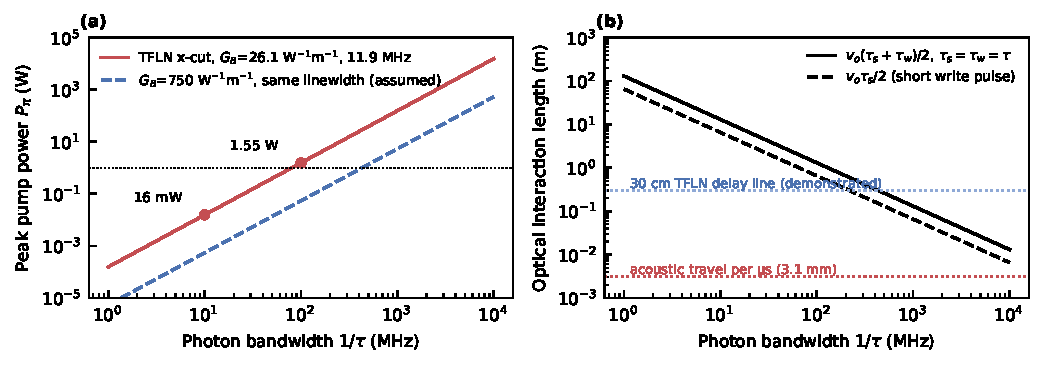
\includegraphics[width=\columnwidth]{figures/fig3_power_length.pdf}
\caption{(a) Peak pump power for a full swap, Eq.~\eqref{eq:Ppi}, versus photon bandwidth $1/\tau$. Points mark 10 and 100~MHz. (b) Optical length of the signal--pump collision region. The acoustic travel per microsecond (3.1~mm) is shown for comparison. Data: \texttt{fig2\_pump\_power.csv}, \texttt{derived\_numbers.json}.}
\label{fig:power}
\end{figure}

%=====================================================================
\section{Storage efficiency and noise}\label{sec:noise}
%=====================================================================
Figure~\ref{fig:storage} evaluates Eq.~\eqref{eq:F} with $\tau_w=10$~ns. At room temperature the SBS phonon has $n_{th}\approx768$ and $\Gamma/2\pi=11.9$~MHz. The fidelity sits at 0.50 for all storage times, so single photons cannot be stored. At 4~K, the 0.7-dB/mm loss gives $\Gamma/2\pi=79.5$~kHz ($1/\Gamma=2.0~\mu$s), $\eta(1~\mu{\rm s})=0.60$, a half-efficiency time of 1.38~$\mu$s, and a delay--bandwidth product of 138. The residual $n_{th}=9.9$, however, limits the fidelity to 0.976 for $t\to0$, to $F>0.9$ for storage up to 40~ns, and to $F>2/3$ up to 0.36~$\mu$s. For comparison, Ref.~\cite{ZhuGenesStiller2026} reports a fidelity of 0.79 at 1~K and 50~ns for its chalcogenide parameters. At 20~mK ($n_{th}\approx5\times10^{-9}$) the fidelity exceeds 0.99 over the whole computed range up to 10~$\mu$s. This result rests on the \emph{assumption} that the 4-K acoustic loss carries over to millikelvin temperatures, which has not been measured for TFLN. In this regime the efficiency, not the fidelity, is the binding constraint: $\eta$ falls to 0.60 at 1~$\mu$s and to $7\times10^{-3}$ at 10~$\mu$s.

\begin{figure}[t]
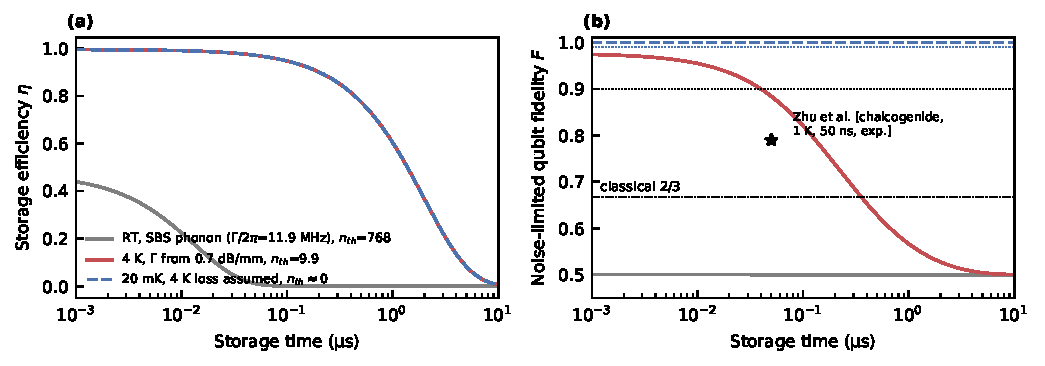
\includegraphics[width=\columnwidth]{figures/fig4_storage.pdf}
\caption{(a) Storage efficiency and (b) noise-limited qubit fidelity, Eq.~\eqref{eq:F}, with ideal swaps and $\tau_w=10$~ns. The 20-mK curve assumes the 4-K acoustic loss (unmeasured). The star marks the value reported in Ref.~\cite{ZhuGenesStiller2026} (chalcogenide, 1~K, 50~ns) and is shown only as a reference point. Data: \texttt{fig3\_storage.csv}.}
\label{fig:storage}
\end{figure}

%=====================================================================
\section{Multimode operation}\label{sec:multimode}
%=====================================================================
\subsection{Local single-acoustic-mode model}\label{sec:local}
In the local limit ($\kappa=0$) only the resonant pairs $n=m$ survive time averaging over $\tau_w$. Equation~\eqref{eq:B} then couples the phonon to the single collective mode $a_w=\sum_n w_n^*A_n$, so the comb weights select which superposition is stored. Integrating Eqs.~\eqref{eq:A}--\eqref{eq:B} for one phonon mode and $N$ bins, including the off-resonant $n\neq m$ terms and the $n\epsilon\Delta$ dispersion, with discrete-Fourier-transform (DFT) target modes, we obtain the storage matrix $E_{kj}$ and the selectivity $\eta_k/\sum_jE_{kj}$ (Fig.~\ref{fig:local}). The selectivity exceeds 0.998 for $\Delta\tau_w/2\pi\ge8$. For $N=8$ and $\tau_w=1$~ns at 10~GHz spacing, both the mean storage efficiency and the mean selectivity are 0.9988. For large $\Delta\tau_w$ the selectivity degrades again (0.9967 at $\Delta\tau_w/2\pi=128$, $N=8$), consistent with the accumulated $n\epsilon\Delta\tau_w$ phase. Note also that $\tau_w=1$~ns corresponds to $P_\pi=155$~W [Eq.~\eqref{eq:Ppi}]. At the watt-level operating point ($\tau_w=10$~ns) the local selectivity lies between the $\Delta\tau_w/2\pi=64$ and 128 values (0.9990 and 0.9967).

\begin{figure}[t]
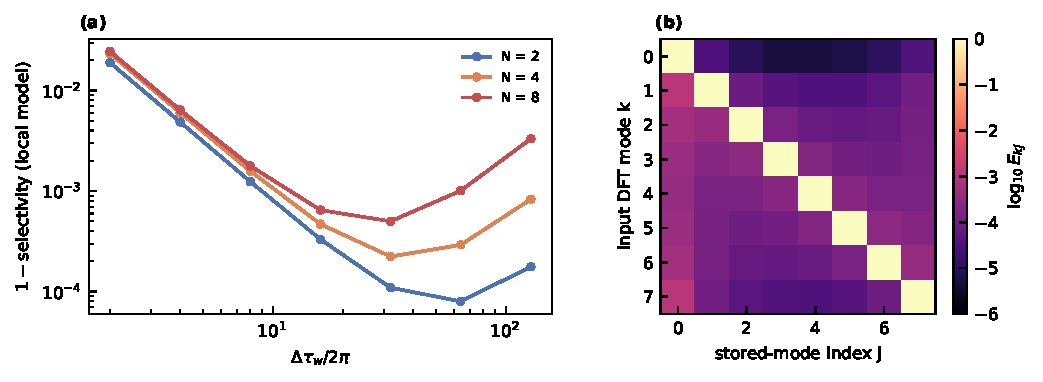
\includegraphics[width=\columnwidth]{figures/fig5_local_multimode.pdf}
\caption{Local (single-acoustic-mode, $\kappa=0$) model. (a) $1-$selectivity versus $\Delta\tau_w/2\pi$ for $N=2,4,8$ bins. (b) Storage matrix $E_{kj}$ for $N=8$, $\tau_w=1$~ns, $\Delta/2\pi=10$~GHz. Section~\ref{sec:phase} shows that this model does \emph{not} describe backward SBS. Data: \texttt{fig4\_multimode.csv}, \texttt{fig4b\_N8\_matrix.csv}.}
\label{fig:local}
\end{figure}

\subsection{Backward-SBS phase matching invalidates the local model}\label{sec:phase}
For $\kappa=1$, the resonant pair $n$ drives the phonon with spatial phase $e^{i2n\Delta z/v_o}$. Different bins therefore write gratings separated by
\begin{equation}
\Delta q=\frac{2\Delta n_g}{c}\approx 964~{\rm rad/m}\quad(\Delta/2\pi=10~{\rm GHz}),\label{eq:dq}
\end{equation}
a spatial beat period of 6.5~mm. The relevant length is the collision region $L_c$ of Sec.~\ref{sec:length}, which is also the length of the written grating. It is not the acoustic wavelength scale $v_{ac}\tau$ ($\sim3~\mu$m). The original concept used the latter length and obtained $\Delta q\,\ell\approx3\times10^{-3}$, but the correct product is $\Delta q\,L_c\simeq2\Delta\tau$. This is $\approx126$ for $\tau=1$~ns and $\approx1.3\times10^3$ for 10~ns. Because the local model itself requires $\Delta\tau_w\gg1$ for frequency resolution, resolved bins in backward SBS always write mutually orthogonal gratings. The phonon field is then $B(z)=\sum_n w_n^*e^{i2n\Delta z/v_o}b_n(z)$, with one independent amplitude per bin. This is exactly the mechanism behind the crosstalk-free multi-wavelength storage of Ref.~\cite{Stiller2019}.

To check this numerically we integrated Eqs.~\eqref{eq:A}--\eqref{eq:B} on a space--time grid. The signal is advected exactly, the pump is undepleted, $\Gamma\to0$, and only the resonant ($n=m$) beats are kept. We used $N=2$, $\tau_s=3$~ns, $\tau_w=1$~ns, $w=(1,1)/\sqrt2$, and a pump area that gives $\eta=0.93$ in the local model. Figure~\ref{fig:spatial} scales the spatial phase by $\kappa$. At $\kappa=0$ the target mode $(a_0+a_1)/\sqrt2$ is stored with $\eta=0.926$ and the orthogonal mode is not stored. Including the off-resonant terms gives $1.1\times10^{-4}$, reproducing the local result. The selectivity falls below 0.99 already at $\Delta qL_c\approx0.08$. At the physical value $\Delta q L_c=251$ ($\kappa=1$) the target and orthogonal modes are stored equally ($\eta=0.821$ each) and the selectivity is 0.500. A single pump line ($w=(1,0)$) stores bin~0 with $\eta=0.926$ and leaves bin~1 untouched ($<10^{-7}$), confirming bin-selective, not superposition-selective, writing.

The read step is equally constrained. A grating $q_{nn}$ read by pump line $m'$ emits at $\omega^p_{m'}+\Omega_B$. Phase matching requires $k_{\rm out}+|k^p_{m'}|=q_{nn}$, and energy and momentum conservation together force $m'=n$, up to corrections of order $\epsilon$. Backward SBS therefore returns each stored component at its original frequency. It cannot remap frequencies, and a read with an ``arbitrary comb combination'' only chooses \emph{which} bins are released, with which amplitude and phase.

\begin{figure}[t]
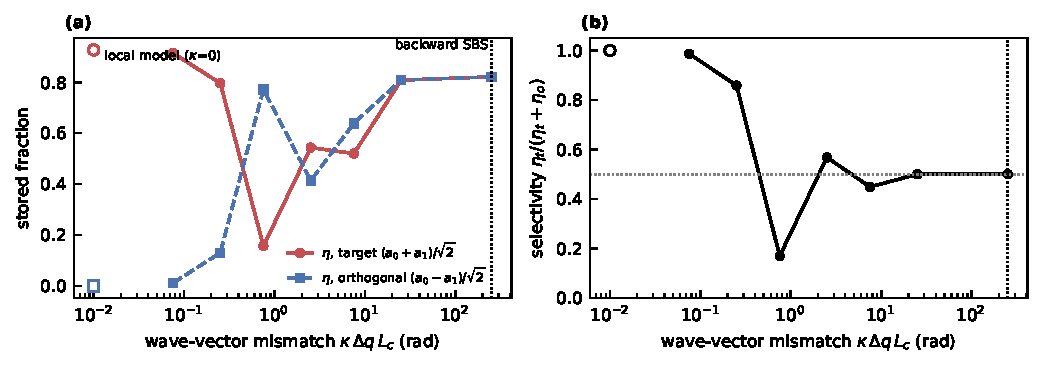
\includegraphics[width=\columnwidth]{figures/fig6_spatial_check.pdf}
\caption{Space--time check of the mode-selective write ($N=2$, $\tau_s=3$~ns, $\tau_w=1$~ns, $\Delta/2\pi=10$~GHz). The spatial phase in Eq.~\eqref{eq:phi} is scaled by $\kappa$; the horizontal axis is $\kappa\Delta qL_c$ with $L_c=v_o(\tau_s+\tau_w)/2=0.26$~m. Open symbols: $\kappa=0$ (local model). Dotted line: physical backward SBS ($\kappa=1$). (a) Stored fraction for the targeted and orthogonal two-bin modes. (b) Selectivity. Data: \texttt{data\_spatial\_scan.json}.}
\label{fig:spatial}
\end{figure}

\subsection{What survives: a bin-diagonal programmable buffer}
In backward SBS the comb therefore acts diagonally in frequency. Each pump line sets, for its own bin, the swap angle (via $|w_n|$), a phase (via $\arg w_n$), and the write and read times. This supports two functions:
\begin{itemize}
\item \emph{Per-bin programmable delay}, i.e.\ time reordering of frequency components. This is a permutation in time, not in frequency.
\item \emph{Synchronization} of photons that arrive in different bins at different times, by firing each bin's line at that photon's arrival and all lines together at readout.
\end{itemize}
Frequency-bin superpositions are stored coherently, as $N$ independent gratings. Each fully swapped bin needs its own line at $P_\pi$, so simultaneous operation of $N$ bins needs $NP_\pi$ in total, for example 12.4~W for $N=8$ at 100~MHz. Mode-selective storage or frequency remapping would require all pairs to address the \emph{same} acoustic mode, i.e.\ $\Delta q L_c\lesssim0.1$ (Fig.~\ref{fig:spatial}). Forward intra- or intermodal Brillouin scattering has $\Delta q\approx0$ or an engineered $\Delta q$. A forward-Brillouin ``super-$\pi$'' pulse that swaps one phonon with an arbitrary frequency-bin superposition, and performs quantum frequency translation through the phonon, has already been proposed~\cite{ShepherdBehunin2025}. A TFLN implementation of that geometry is not evaluated here.

%=====================================================================
\section{Relation to prior work and novelty}\label{sec:prior}
%=====================================================================
Table~\ref{tab:compare} positions the reduced PFB among related approaches. Classical Brillouin storage in chalcogenide chips~\cite{Merklein2017,Stiller2020,Stiller2024} and in fiber~\cite{ZhuGauthierBoyd2007,Geilen2024,Saffer2025,Zeng2026} established coherent storage. Multi-wavelength, crosstalk-free operation~\cite{Stiller2019} already demonstrated the bin-diagonal function that survives our analysis. The quantum-regime analysis of Ref.~\cite{ZhuGenesStiller2026} treats a single optical mode. Superposition-selective swaps and frequency translation via a phonon have been proposed for forward Brillouin~\cite{ShepherdBehunin2025}. Acousto-optic intermodal frequency beam splitters (FRODO) give universal frequency-bin unitaries but no storage~\cite{Lukens2026FRODO}. Outside Brillouin physics, a Raman memory in warm vapor already performs mode-selective storage, filtering and conversion of 30 temporal modes~\cite{Zhang2026Raman}. Spectrally multiplexed atomic-frequency-comb memories~\cite{Sinclair2014} and a recent proposal for frequency-bin synthesis in a rare-earth memory~\cite{Moiseev2026} address frequency bins with different physics. TFLN SBS has been characterized for gain, lasing, and RF photonics~\cite{Ye2023SAW,Ye2025SciAdv,Rodrigues2025,Haerteis2025}, and IDT-driven backward-Brillouin coupling has been demonstrated in LN-on-sapphire rings~\cite{Xu2025LNOS,Zhu2025LNOS}. We found no report of Brillouin optical \emph{storage} in TFLN, or of an EO-comb-pumped Brillouin frequency-bin memory. The contributions of this work are therefore limited to (i) TFLN-specific delay, power and noise budgets; (ii) the explicit space--time demonstration that comb-programmed superposition selection fails in backward SBS; and (iii) the interaction-length constraint on footprint. We regard the novelty as moderate, and lower than originally envisaged.

\begin{table*}[t]
\footnotesize
\caption{Comparison with related frequency/temporal-mode processors and memories. Values are as reported in the cited works. ``This work'' rows are simulations.}
\label{tab:compare}
\begin{ruledtabular}
\begin{tabular}{p{3.6cm}p{3.0cm}p{1.4cm}p{4.4cm}p{4.2cm}}
Approach & Platform & Storage & Mode/bin operation & Reported metrics\\ \hline
\raggedright PFB, local model (this work)&\raggedright TFLN, backward SBS&\raggedright yes (sim.)&\raggedright superposition-selective (invalid, Sec.~\ref{sec:phase})&\raggedright sel.\ 0.9988 ($N=8$)\tabularnewline
\raggedright PFB, space--time (this work)&\raggedright TFLN, backward SBS&\raggedright yes (sim.)&\raggedright bin-diagonal: per-bin delay/phase&\raggedright sel.\ 0.50 ($N=2$); 2.2~\dBus{} (4~K)\tabularnewline
\raggedright EO QFP~\cite{Lu2018PRL}&\raggedright fiber EOM + shaper&\raggedright no&\raggedright arbitrary unitaries&\raggedright Hadamard $F=0.99998$, $P=0.9739$\tabularnewline
\raggedright Double-ring f-BS~\cite{Yang2026QFP}&\raggedright TFLN, EO&\raggedright no&\raggedright 2-bin BS, CZ&\raggedright 1-qubit $97.1\%$, CZ $91.4\%$\tabularnewline
\raggedright QPG~\cite{Babel2026QPG}&\raggedright TFLN, SFG&\raggedright no&\raggedright temporal-mode selection&\raggedright sel.\ $96.8\%$ / $91.7\%$ (1 photon)\tabularnewline
\raggedright FRODO~\cite{Lukens2026FRODO}&\raggedright Si/SiN, intermodal AO&\raggedright no&\raggedright universal unitaries (theory)&\raggedright 7-GHz bins\tabularnewline
\raggedright Forward super-$\pi$~\cite{ShepherdBehunin2025}&\raggedright forward Brillouin&\raggedright phonon&\raggedright superposition swap, QFT (theory)&\raggedright ---\tabularnewline
\raggedright Raman TM processor~\cite{Zhang2026Raman}&\raggedright warm Cs vapor&\raggedright yes&\raggedright 30 HG modes, conversion&\raggedright 5D process $F=0.943$\tabularnewline
\raggedright Brillouin quantum memory~\cite{ZhuGenesStiller2026}&\raggedright chalcogenide (theory)&\raggedright yes&\raggedright single mode&\raggedright $F=0.79$ (1~K, 50~ns)\tabularnewline
\end{tabular}
\end{ruledtabular}
\end{table*}

%=====================================================================
\section{Limitations}\label{sec:limits}
%=====================================================================
The conclusions above are subject to the following limitations, which we consider essential:
\begin{enumerate}
\item \emph{The acoustic loss of TFLN at millikelvin temperatures is unmeasured.} All 20-mK results assume the 4-K value of 0.7~dB/mm.
\item \emph{Frequency mismatch of the loss data.} The 0.7-dB/mm (4~K) and 4.0-dB/mm (RT) values were measured at $\approx3.4$~GHz in LN-on-sapphire phononic waveguides~\cite{Mayor2021}. The backward-SBS phonon is at $\approx8$--9~GHz in a different (SAW-like) mode of a TFLN optical waveguide~\cite{Ye2023SAW}. Acoustic loss generally increases with frequency, so the 8-GHz loss may be substantially larger than assumed.
\item \emph{Not computed:} pump-induced heating (which would raise $n_{th}$ above the bath value, critically at 20~mK with watt-level pumps), spontaneous Stokes and anti-Stokes noise generated by the pump, and chip coupling loss. Off-resonant $n\neq m$ crosstalk is included only in the local model.
\item The meter-scale collision region (Sec.~\ref{sec:length}) requires long, low-loss waveguides that guide the 8-GHz phonon throughout. Such waveguides have not been demonstrated, and their optical loss (e.g.\ $\approx1.3$--2.5~dB/m) adds a fixed insertion loss that is not included in $\eta$.
\item $n_g=2.3$, $\Delta/2\pi=10$~GHz, ideal $\pi$-swaps, undepleted pumps, and the absence of acoustic diffraction and dispersion are assumptions. The space--time check uses $N=2$ and $\Gamma\to0$ and does not optimize pulse shapes.
\end{enumerate}

%=====================================================================
\section{Conclusion}
%=====================================================================
A comb-pumped backward-SBS buffer in TFLN offers a compact, IDT-free acoustic delay that, at 4~K, is an order of magnitude less lossy per microsecond than the best TFLN optical lines but still worse than fiber. Its pump power restricts it to $\sim$10--100-MHz photons, and its noise restricts single-photon use to cryogenic, and realistically millikelvin, operation. Programmable selection of frequency superpositions, the central premise of the concept, is incompatible with backward-SBS phase matching. The device is instead a bin-diagonal memory with per-bin delay, phase and swap control, already anticipated classically by multi-wavelength Brillouin storage. Mode-selective storage would require a forward-Brillouin geometry, which we leave to future work. Measurements of 8-GHz acoustic loss at millikelvin temperatures, and of pump-induced heating, are the decisive experimental inputs.

\section*{Data and code availability}
All scripts and data are provided with the manuscript: \texttt{scripts/simC.py} and \texttt{params.py} (original model), \texttt{paper/scripts/make\_figs.py} (figures and derived numbers), and \texttt{paper/scripts/spatial\_check.py} and \texttt{spatial\_scan.py} (space--time check).

\bibliography{refs}

\end{document}
